% vim:ft=tex
\section{The model}
\label{sec:the-model}
%	There should be an introduction here. What will the reader learn during the section. 	%


\subsection{Explanation of our model}
In this section we will elaborate on the construction of the model from the article \cite{self-org} in great detail. 
First of all, as stated briefly earlier this model is an agent based social force model. 
This means that the model uses individual entities to say something about the collective behaviour of the crowd. 

Each entity or agent is acted on by a collection of different forces, and the agent cannot escape 
from Newton's three laws about the motion of any object, which mainly says that when there is a 
force it results in a corresponding acceleration.  However, our agent is not a ball being kicked around, 
it has a willingness to go to some destine place.  The way that the will is implement in an agent is by 
generating a statistic frictional force from the ground, and that force is here what we called 
the social force.

\begin{figure}[hb]
    \centering
    {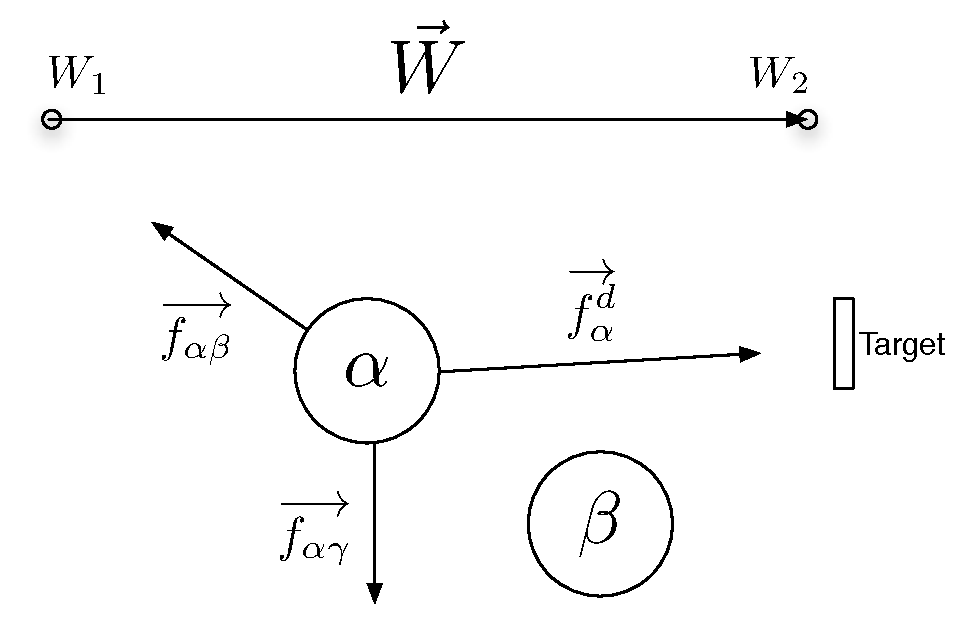
\includegraphics[scale=0.45]{Figures/ForceModel.pdf}} 
    \caption{}
    \label{ForceModel}
\end{figure}

These forces can be either repulsive or attractive. The general approach of the model 
is fairly simple. An agent $\alpha$ wants to go in a desired direction with a desired speed. 
However the environment and other agents might force agent $\alpha$ to stray from the desired 
direction or have speeds different from the desired one. The change in position of 
agent $\alpha$ is given by:

\begin{equation}
		\frac{d \vec{r_{\alpha}}}{dt} = \vec{V_{\alpha}} \left( t \right)
\end{equation}

Where $\vec{V_{\alpha}} \left( t \right)$ is the velocity of agent $\alpha$ at time t.
And, as we know from newtonian physics that, the acceleration of agent $\alpha$ is given by the summation of all the forces acting on the agent:

\begin{equation}
    \frac{d \vec{V_{\alpha}}}{dt} = \vec{f_{\alpha}} \left( t \right) 
\end{equation}

$\vec{f_{\alpha}} \left( t \right)$ is a summation of all the forces acting on 
agent $\alpha$ from the environment and other agents. More specifically it is given by:

\begin{equation}\label{model}
    \vec{f_{\alpha}} = \vec{f^{0}_{\alpha}}\left( \vec{V_{\alpha}} \right) + 
    \vec{f_{\alpha B}} \left( \vec{r_{\alpha}} \right) +
    \sum_{\beta \neq \alpha} \vec{f_{\alpha \beta}} \left(\vec{r_{\alpha}}, 
    \vec{V_{\alpha}}, \vec{r_{\beta}}, \vec{V_{\beta}} \right) +
    \sum_{i} \vec{f_{\alpha i}} \left( \vec{r_{\alpha}}, \vec{r_{i}}, t 
    \right)
\end{equation}

$\vec{f^{0}_{\alpha}}\left( \vec{V_{\alpha}} \right)$ is an acceleration force. $\vec{f_{\alpha B}} \left( \vec{r_{\alpha}} \right)$ is a repulsive force arising from boundaries. $\sum_{\beta \neq \alpha} \vec{f_{\alpha \beta}} \left(\vec{r_{\alpha}}, \vec{V_{\alpha}}, \vec{r_{\beta}}, \vec{V_{\beta}} \right)$ is a repulsive force due to other agents obstruction agent $\alpha$.
This is a summation of four different kinds of forces. We will go through 
them one at a time explaining their role in the model and their mathematical 
structure.\\

\begin{figure}[hb]
    \centering
    {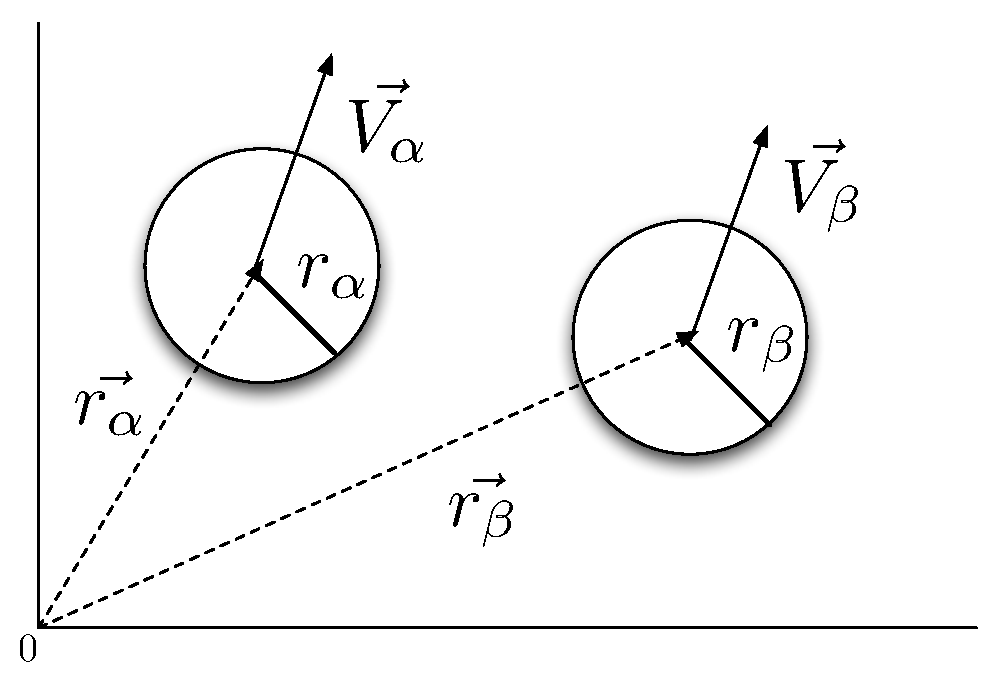
\includegraphics[scale=0.35]{Figures/NotationOAgent.pdf}} 
    \caption{Shows a visual presentation of the mathematical notation.}
    \label{NotationOAgent}
\end{figure}

\subsubsection{The velocity dependence} %gotta figure out a better name for this part
The first term on the right hand side of equation \eqref{model} is a velocity dependent force 
and it is given by:

\begin{equation}
	\vec{f^{0}_{\alpha}}\left( \vec{V_{\alpha}} \right) =
    \frac{1}{\tau}
    \left( V_{\alpha}^{0} \vec{e_{\alpha}} - \vec{V_{\alpha}} \right)
\end{equation}

Here $\tau$ is the relaxation time. % lets go a little more into detail about this relaxation time. We discussed it with viggo last time
$\vec{V_{\alpha}}$ is the  current velocity of the agent and $V_{\alpha}^{0}$ 
is the initial speed, that is the speed of the agent at the end of the last 
simulation step. $V_{\alpha}^{0}$ is given by:

\begin{equation}\label{v0}
    V_{\alpha}^{0} = \left[ 1 - \eta_{\alpha} \left( t \right) \right] 
    V_{\alpha}^{0} \left( 0 \right) +
    \eta_{\alpha} \left( t \right)V_{\alpha}^{\text{max}}
\end{equation}

Here $V_{\alpha}^{0} \left( 0 \right)$ is the velocity at time $t=0$ and $V_{\alpha}^{\text{max}}$ is the maximum desired speed of agent $\alpha$, the agent can desire a lower speed but the value of the desired speed can at most be $V_{\alpha}^{\text{max}}$. The agent can have a higer speed than $V_{\alpha}^{\text{max}}$ but then the agent will attempt to slow down to reach his desired speed. $\eta_{\alpha}$ is called the impatience or nervousness of the agent and is given by:

\begin{equation}
	\eta_{\alpha} \left( t \right) =
    1 - \frac{\overline{V}_{\alpha} \left( t \right)}
             {V_{\alpha}^{0} \left( t \right)}
\end{equation}

Here $\overline{V}$ is the average speed in the desired direction and as 
earlier $V_{\alpha}^{0} \left( 0 \right)$ is the initial speed. $\eta_{\alpha}$ is called the impatience 
or nervousness factor of agent $\alpha$ and we will a little time on it her because 
it does yield some interesting dynamics. 

First of all The impatience or nervousness factor is active when one calculates the 
force action on agent $\alpha$ from the velocity of the agent.

In the case where $0 \leq \eta_{\alpha} \leq 1$ the expression for 
$V_{\alpha}^{0} \left( t \right)$  makes sense. Here we can see why this term 
is called the impatience of the agent. If the fraction  between the average 
speed in the desired direction and the initial speed is low then $\eta_{\alpha} \approx 1$. 
When the impatience term is close to one $V_{\alpha}^{0} \left( t \right)$ 
is dominated by $V_{\alpha}^{\text{max}}$. That is, if the agent have not 
moved very far in the desired direction compared to the initial speed the 
impatience of the agent will cause the agent's future velocity to be dominated by 
the desired velocity of the agent.

If the agent has been moving in the desired direction with his initial 
speed the entire time then $\eta_{\alpha} = 0$  and 
$V_{\alpha}^{0} \left( t \right)$ will continue to be $V_{\alpha}^{0} \left( 0 \right)$.

In the case where $\eta_{\alpha} \leq 0$ that is the agent has moved further 
in the desired direction then he would have had he been walking with his 
initial speed. The expression for $V_{\alpha}^{0} \left( t \right)$
stats yield strange results. That $\eta_{\alpha} \leq 0$ would imply that:

\begin{equation}\label{n}
    V_{\alpha}^{0} = \left[ 1 + \eta_{\alpha} \left( t \right) \right] 
    V_{\alpha}^{0} \left( 0 \right) -
    \eta_{\alpha} \left( t \right)V_{\alpha}^{\text{max}}
\end{equation}

And this will yield a negative value for $V_{\alpha}^{0}$ if: 

\begin{equation}
\left[ 1 + \eta_{\alpha} \left( t \right) \right] 
V_{\alpha}^{0} \left( 0 \right) < \eta_{\alpha} \left( t \right)V_{\alpha}^{\text{max}} 
\end{equation}

This is a problem because it is not that far fetched that an agent will be 
forced to exceed his desired velocity.

In the case where $1 \leq \eta_{\alpha}$ it would mean that the agent has moved 
further in the opposite direction than the desired one and this can only happen very 
weird situations.

Equation (\ref{n}) and Equation (\ref{v0}) contains an intermediate variable $ n_{\alpha} \left( t \right) $, 
so in principle we are allowed to eliminate $ n_{\alpha} \left( t \right) $ and only show the 
relationship between $ V_{\alpha}^{0}(t) $ and $ \overline{V}_{\alpha} \left( t \right) $. Thus we get:

\begin{equation}\label{vv}
    V_{\alpha}^{0}(t) = \left[ 1 - \frac{v_{\alpha}^{max}}{v_{\alpha}^{0}(0)}\right]\overline{V}_{\alpha} \left( t \right) + v_{\alpha}^{max}
\end{equation}

\begin{figure}[ht]
\centering
{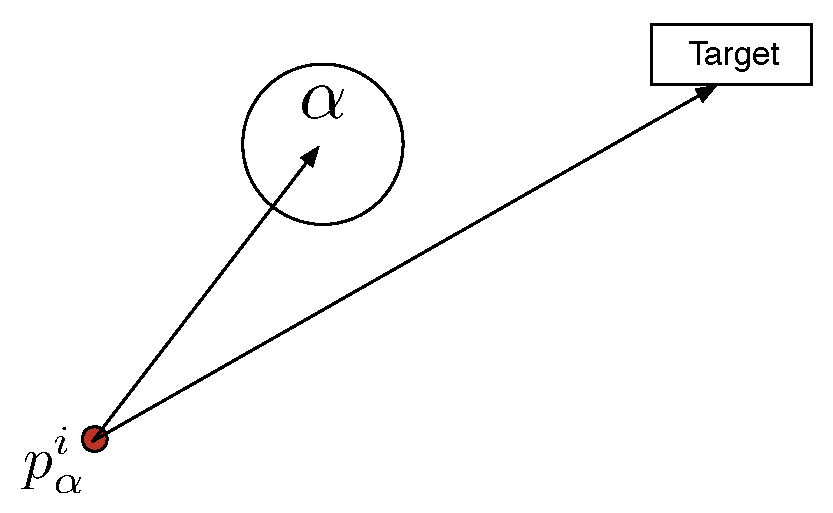
\includegraphics[scale=0.35]{Figures/impatience.pdf}} 
\caption{\small{The function about the desired velocity $ V_{\alpha}^{0}(t) $ 
and the average velocity in the desired direction of motion $ \overline{V}_{\alpha} \left( t \right) $}}
\label{impatience}
\end{figure}

Figure (\ref{impatience}) is a drawing of the graph about those two variables, and the intersection
 of the function line with both axis are:

\begin{equation}
\left( 
	\overline{V_{\alpha}} , V_{\alpha}^{0} \left( t \right)
\right)
=
\left( 
	0 
		, 
	v_{\alpha}^{max} 
\right) 
\text{and} 
\left(
	v_{\alpha}^{max} 
		\frac{v_{\alpha}^{0} \left( 0 \right) }{v_{\alpha}^{max}-v_{\alpha}^{0} \left(0 \right)} 
	, 0 
\right) 
\end{equation}
Now there is a doubt whether the value of $ \overline{V}_{\alpha} \left( t \right) $ can reach $ v_{\alpha}^{max}\frac{v_{\alpha}^{0}(0)}{v_{\alpha}^{max}-v_{\alpha}^{0}(0)} $, if we have already 
set $ v_{\alpha}^{max} $ a fixed number for a certain agent. In the case:

\begin{equation}
	v_{\alpha}^{max} 
	\geq 
	v_{\alpha}^{max} 
	\frac{v_{\alpha}^{0}(0)}{v_{\alpha}^{max}-v_{\alpha}^{0}(0)}
\end{equation}

we get the relation:

\begin{equation}
v_{\alpha}^{0}(0)\leq \frac{1}{�2}v_{\alpha}^{max}
\end{equation}

% Lets have a little summation here. What have we learned about the inpatience factor and
% the velocity dependant force. What kind of dynamics does this force yield

\subsubsection{Interaction with the walls}
Now the second term on the right hand side of \eqref{model} is the forces acting on agent 
$\alpha$ from the walls of the room. The force is given by:

\begin{equation}
    \vec{f_{\alpha B}} \left( \vec{r_{\alpha}} \right) =
    - \nabla_{\vec{r_{\alpha}}} V_{B}
    \left( \| \vec{r_{\alpha}} - \vec{r_{B}^{\alpha}} \| \right)
\end{equation}

Here $\nabla_{\vec{r_{\alpha}}}$ is the gradient of $V_B$, which is a repulsive 
potential. $V_B$ is only dependent on $ \| \vec{r_{\alpha}} - \vec{r_{B}^{\alpha}} \|$ which is the distance 
from agent $\alpha$ to the nearest point of the nearest wall.

\begin{figure}[ht]
\centering
{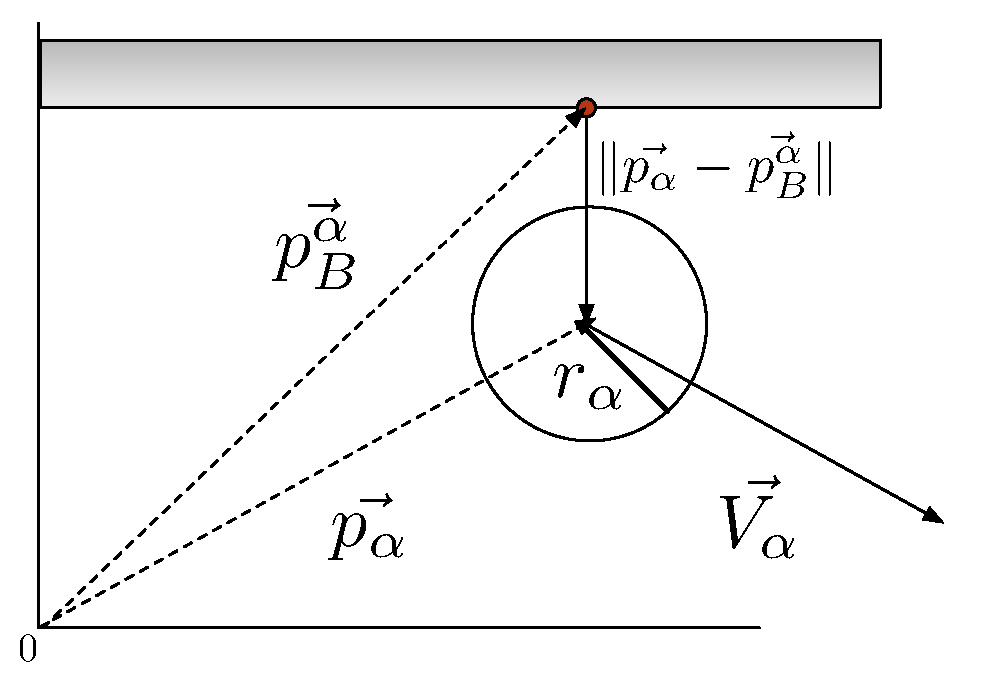
\includegraphics[scale=0.35]{Figures/NotationOfWall.pdf}} 
\caption{\small{Shows the notation for the interaction with walls.}}
\label{NotationOfWall}
\end{figure}

The repulsive potential describes the force added from the walls to pedestrian $\alpha$, since $\alpha$ does not
want to get too close to the wall. So the closer $\alpha$ get to the wall the more the force from the wall gets.
The repulsion potential is given by:

\begin{equation}
V_{B} \left( \| \vec{r_{\alpha}} - \vec{r_{B}^{\alpha}} \| \right) =
V^0_{\alpha B} e^{- \| \vec{r_{\alpha}} - \vec{r_{B}^{\alpha}} \| / r_{\alpha} }
\end{equation}

Here $V^0_{\alpha B}$ is a constant and $r_{\alpha}$ is the radius of a pedestrian $\alpha$.

The reason for this repusion force from the wall is that the pedestrians do not want to get hurt by running into the walls
or get crushed between the panicing crowd and the wall [Helbing and Molnár, 1995]. %real references, please.

\subsubsection{Interaction between agents}
The third term on the right hand side of \eqref{model} is a summation of all the 
force between agent $\alpha$ and agent $\beta$. It is a function of the position vector and the velocity of 
both agents, and it is given by:

\begin{equation}
    \sum_{\beta \left( \neq \alpha \right)}
        \vec{f_{\alpha \beta }}\left( t \right) =
        A_{\alpha}^{1} exp \left(
            \frac{ r_{\alpha \beta} - d_{\alpha \beta }}
                 {B_{\alpha}^1}
        \right)
    \vec{\eta_{\alpha \beta}} \cdot
    \left(
        \lambda_{\alpha} + \left(
            1 - \lambda_{\alpha}
        \right)
		\frac{1+\cos{\phi}}{2}
    \right) +
    A_{\alpha}^{2} exp\left(
        \frac{r_{\alpha \beta} - d_{\alpha \beta}}
             {B_{\alpha}^{2}}
    \right)
    \vec{\eta_{\alpha \beta}}
    \label{agentinteraction}
\end{equation}

\begin{figure}[ht]
    \centering
    {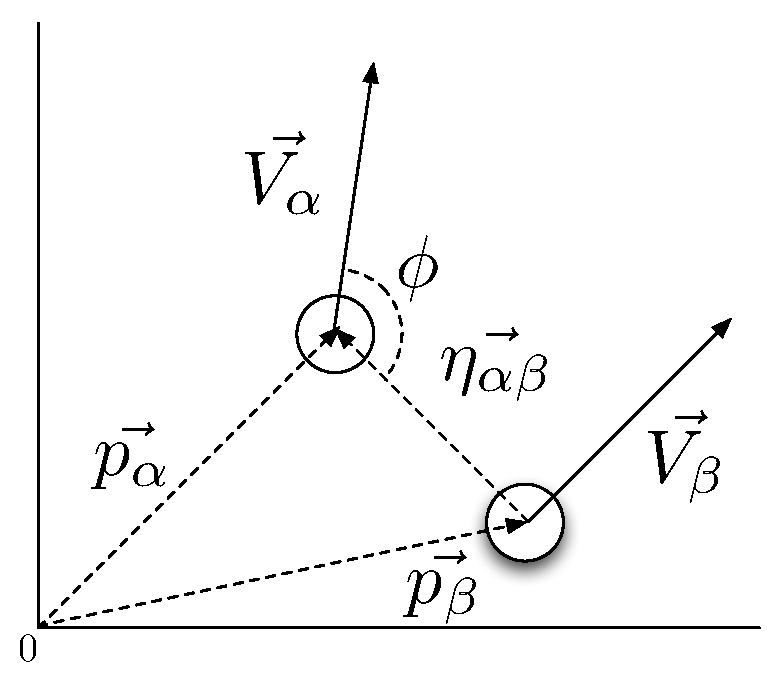
\includegraphics[scale=0.35]{Figures/NotationOfInteraction.pdf}} 
    \caption{Shows the notation for the interaction between agents.}
    \label{NotationOfInteraction}
\end{figure}

Here $A_{\alpha}^{1}$, $A_{\alpha}^{2}$, $B_{\alpha}^{1}$, $B_{\alpha}^{2}$ 
and $\lambda_{\alpha}$ are all constants that can differ for each agent. 
$r_{\alpha \beta}$ is the sum of the radii of $\alpha$ and $\beta$ that is 
$r_{\alpha \beta} = r_{\alpha} + r_{\beta}$. $d_{\alpha \beta}$ is the 
distance from the center of mass of agent $\alpha$ and the center of mass of 
agent $\beta$ and is therefore given by $d_{\alpha \beta} = 
\|\vec{r_{\alpha}}\left( t \right) - \vec{r_{\beta}}\left( t \right) \|$.
$\eta_{\alpha \beta}$ is the normal vector pointing from $\alpha$ to $\beta$ 
and it is given by:

\begin{equation}
    \eta_{\alpha \beta} =
        \frac{\vec{r_{\alpha}}(t) - \vec{r_{\beta}}(t)}
             {\|\vec{r_{\alpha}}(t) - \vec{r_{\beta}}(t) \|}
\end{equation}

the angle $\phi$ in \eqref{agentinteraction} is the angle between the normal 
vector pointing from agent $\beta$ to $\alpha$ and the direction in which 
agent $\alpha$ is moving. Cosine to the angle is 

\begin{equation}
\cos \left( \phi \right)
	\left( t \right) 
		= 
	- \vec{\eta_{\alpha \beta}}
		\left( t \right) 
	\cdot 
\vec{e_{\alpha}}\left( t \right)
\end{equation}

Equation \eqref{agentinteraction} is divided into two terms. The first term on 
the right hand side reflects the agents tendency to stay at a certain distance 
from other agents. This part of the force is called the private sphere because 
the agent prefers to have some free space around him if possible. The radius 
of the private sphere can differ from agent to agent. The constant 
$A_{\alpha}^{1}$, $B_{\alpha}^{1}$ and $\lambda_{\alpha}$ control the nature 
of the private sphere $A_{\alpha}^1$ and $B_{\alpha}^1$ control the strength 
and range of the interaction respectively. $\lambda_{\alpha}$ is there to take 
into account a persons tendency to focus on things happening in front of him 
rather than behind him.	% we should make a drawing of this.

The second term of equation \eqref{agentinteraction} deals with physical interaction.
In the situation where the density of the crowd is high the agents will have be closer
to each other and the social sphere is undermined. % go more into detail here 
So if we look away from the social sphere for a minute and concentrate on the physical
interaction we will see that if we omit the social sphere the calculation will be reduced to
to:

\begin{equation}\label{re}
\overrightarrow{f_{\alpha\beta}}(t) = A_{\alpha}^{2} exp\left[ \frac{r_{\alpha\beta} - d_{\alpha}\beta}{B_{\alpha}^{2}}\right]  \overrightarrow{n_{\alpha\beta}}
\end{equation}

Taking the norms of both sides of Equation (\ref{re}), we can draw the relation between the value of $\overrightarrow{f_{\alpha\beta}}(t)$ and $ d_{\alpha\beta} $, as shown in Figure 
(\ref{physicalinteraction}).\\

\begin{figure}
    \centering
    {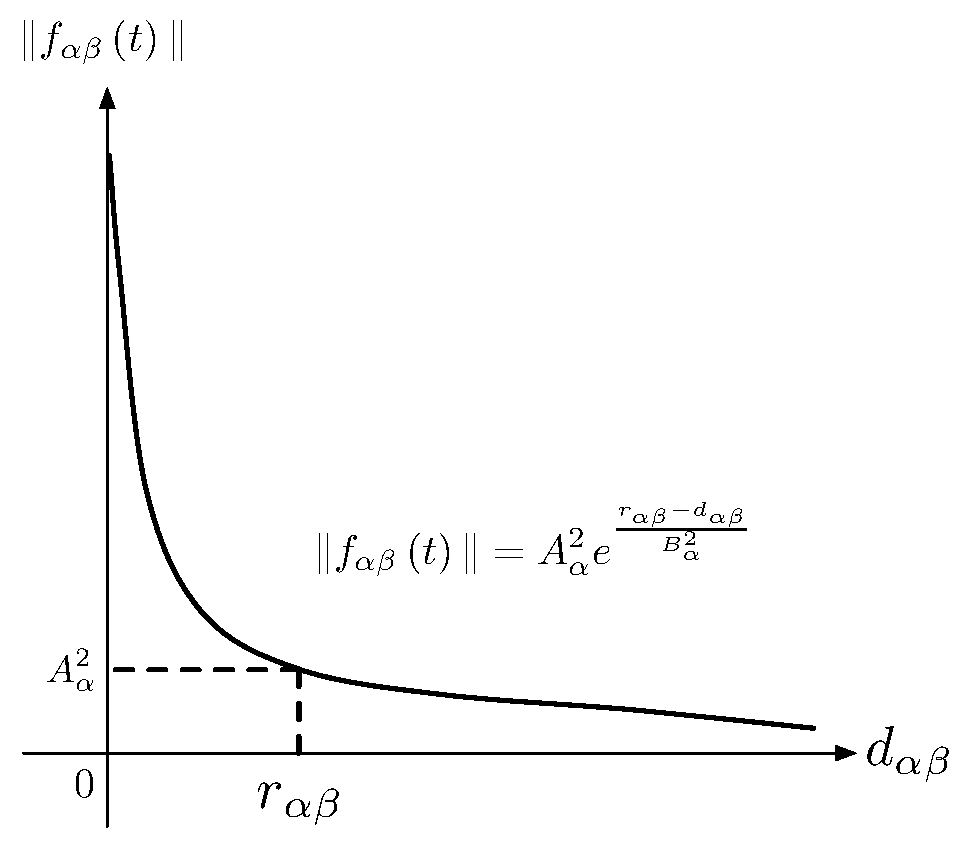
\includegraphics[scale=0.45]{Figures/physicalinteraction.pdf}} 
    \caption{The function about the interaction force 
        $f_{\alpha\beta}(t)$ and the distance between two agents
        $d_{\alpha \beta}$ }
    \label{physicalinteraction}
\end{figure}

There is one intersection of the graph and the  axis at:

\begin{equation}
	\left( d_{\alpha \beta} , \| \vec{f_{\alpha \beta}} \left( t \right) \| \right)
 =
	\left( 0 , A_{\alpha}^{2} exp\left( \frac{r_{\alpha\beta} }{B_{\alpha}^{2}}\right)  \right) 
\end{equation}

If put into the constants, we will be able to get a maximum value of $ f_{\alpha\beta}(t) $, 
since the distance between agents cannot be negative. Here we set $ A_{\alpha}^{2} = 3 m/s^{2} $, 
$ r_{\alpha\beta} = 0.6 m $, and $ B_{\alpha}^{2} = 0.2 m $, so 
$ f_{\alpha\beta}(t)^{max} \doteq 60 m/s^{2} $, which is about six times the gravitational 
acceleration and represents a rather large force between agents (as large as six person's weight).

However, we notice that the effective part of the force calculated above is only the horizontal 
component that enables the agent to move horizontally in the plane where we do the simulation, 
but the reality is that the agents sometimes are also able to move vertically, for example, 
by stepping upon other people when they cannot take the pushing force from the surrounding agents. 
When that happens, the horizontal component of the repulsive force becomes smaller even if $ d_{\alpha\beta} $ 
is kept the same.	

\begin{figure}[ht]   
\centering
    {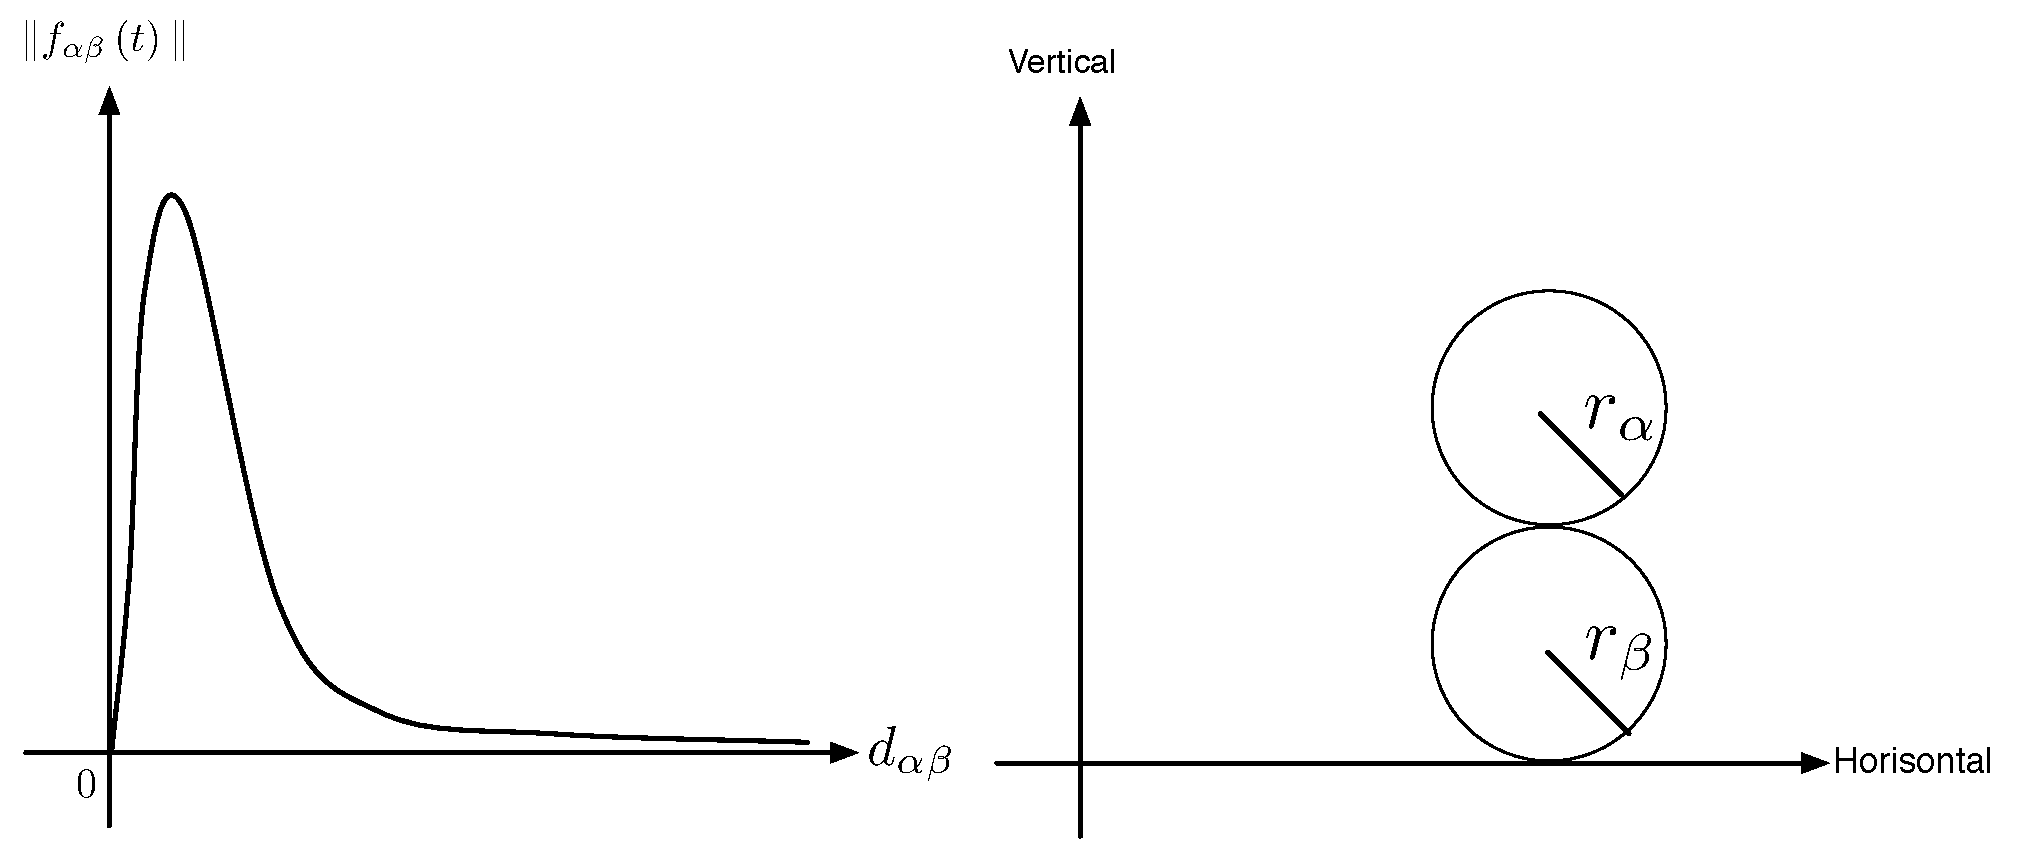
\includegraphics[scale=0.35]{Figures/ForceOverlapping.pdf}} 
    \caption{}
    \label{forceoverlapping}
\end{figure}

Therefore, a qualitative modification of dependence between $ f_{\alpha\beta}(t) $ and $ d_{\alpha\beta} $ could be:
% remember to finish this section

% again lets  have a little summation here. What kinds of dynamics does the
% social interaction part of the model yield.

\subsubsection{The attraction forces}
The fourth and last term in \eqref{model} represents the force from attraction 
in the room. Attractions can be either be either interesting sculptures or 
sights or familiar persons the agent prefer to be close to, such as friends 
and family. The mathematical structure of this force is the same as the force 
from other agents, however it is opposite in algebraic sign and has different 
constants. 

To get an overview of how the model is put together look a figure \ref{overview}
with the aid of table \ref{tableofconstandvar}

\begin{figure}[hb] %with some more comments i think that this figure could serve as a summation of the entire section
    \centering
    {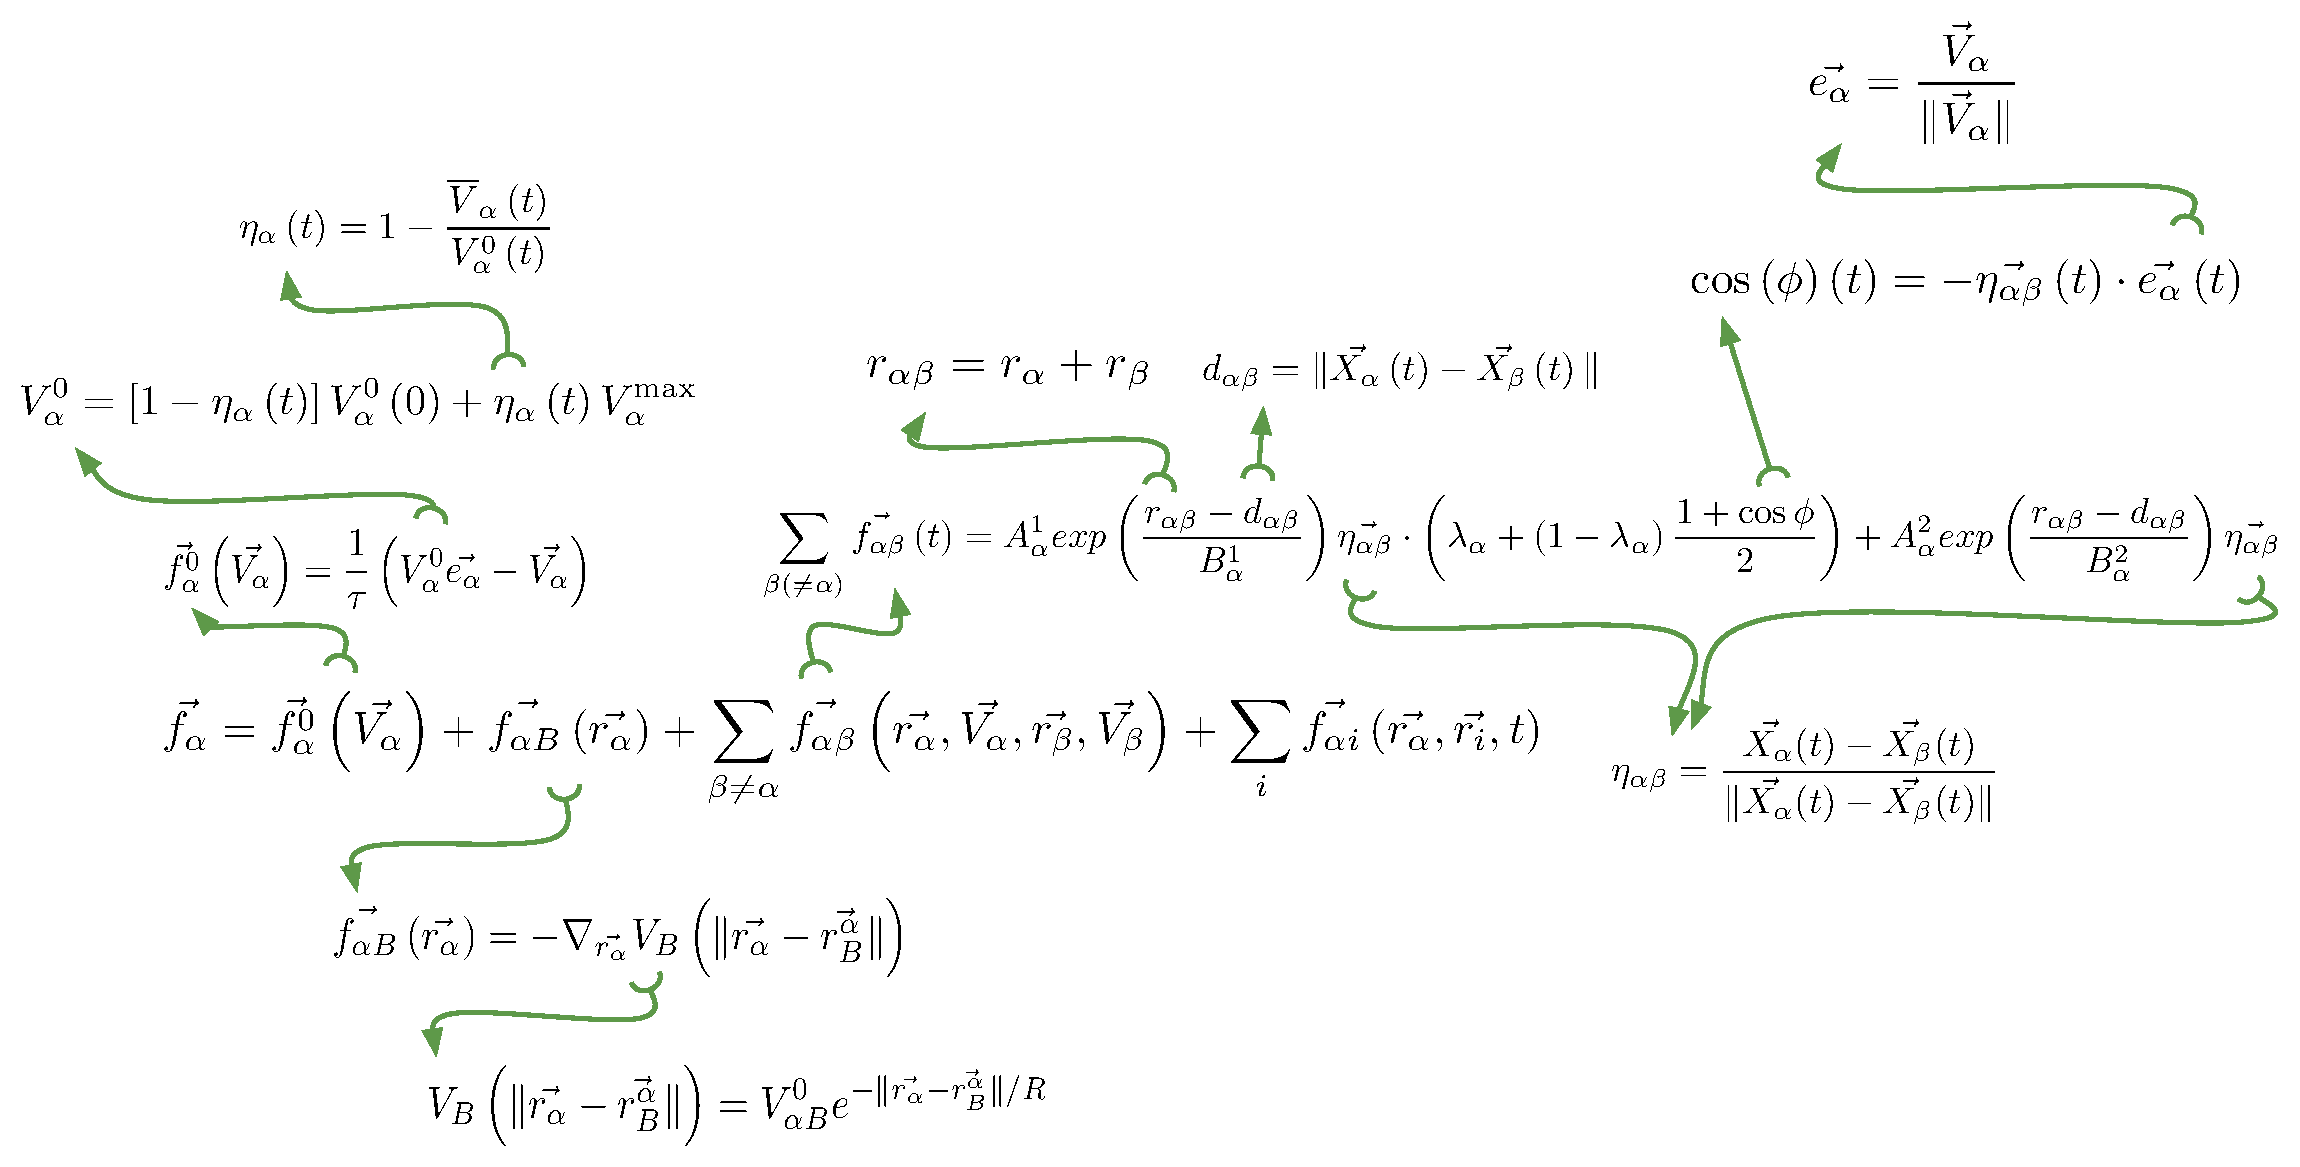
\includegraphics[scale=0.45]{Figures/overview.pdf}} 
    \caption{An overview of how the model is put together}
    \label{overview}
\end{figure}

\clearpage
\section{sec:discussion}\label{sec:discussion}
\subsection{Repulsive force}
In chapter 3 we have seen the formulas for calculating the repulsive forces from the wall and other agents are very similar, both are exponential functions decreasing with some distance, which makes us wonder if both come from the same origin.\\

\begin{itemize}
\item The difference between those two repulsive forces is basically one is from a single point and the other is from an object that has a dimension much larger than a single agent. If we imagine our agents are particles with negative charge, then there is a pair of repulsive forces which has direction along the line connecting the two particles and magnitude depending on the distance between them. Further we can put lots of particles along a bar, see Figure
Summing up all the repulsive forces from each particle on the bar will give the repulsive force that the charged bar on the single particle $\alpha$.

\item Applying the idea above to analyse our wall repulsion, as a simple start we place the agent $\alpha$ a distance $ d $ away from the wall which as a length $L$, and by symmetry we know the resulting force must point vertically downwards, see Figure.\\

Integrating the forces can be written as:

\begin{equation}\label{integ}
\vec{f_{\alpha B}} = 
\int_0^L \! \vec{f_{\alpha\beta}} \, \mathrm{d}l
\end{equation}

\item When the repulsive force is known, the expression for the wall potential can be calculated, which can be done by integrating the force along a path. Normally the potential at some position is defined as the work done on the particle by that potential field when the particle is moved from that position to infinitely far away.

\begin{equation}\label{pot}
	U_{B}= \int_{\vec{r_{\alpha}}�}^{text{f}\infty} \! \vec{f_{\alpha B}} \cdot \, \text{d}\vec{r_{\alpha}} 
\end{equation}

\item In some article [Helbing 2000], the repulsive force from the wall is given by:
\begin{equation}\label{helbing2000}
\vec{f_{\alpha B}} = 
	\left( 
			\left[ 
	A exp 
				\left[ 
						\left(  
							r_{\alpha}-d_{\alpha B}
						\right)  / B
				\right] +kg 
					\left( 
						r_{\alpha}-d_{\alpha B} 
					\right) 
			\right] 
		\right)
	\vec{n_{B}^{\alpha}}-\kappa g 
	\left(
		r_{\alpha}-d_{\alpha B}
	\right) 
	\left(
			\vec{V_{\alpha}}\cdot \vec{t_{iw}}
	\right) 
\vec{t_{iw}}
\end{equation}

where $ r_{\alpha} $,  $ \vec{V_{\alpha}} $ are the radius and velocity of agent $ \alpha $ as we noted before, $ A $, $ B $, $ k $, $ \kappa $ are constants, $ d_{\alpha B} $ is the distance from the agent to the wall, $ \vec{n_{B}^{\alpha}} $ is a normal vector from the wall, $ \vec{t_{iw}} $ is a tangent vector to the wall. $ g $ is a function of some variable.\\
In this expression, the wall repulsion force to agent $ \alpha $ is not always perpendicular to the wall, but the force has two components, one perpendicular to the wall and the other tangent to the wall. Particularly the tangent component depends on the velocity of $ \alpha $. However, in Helbing's latest articles he does not show the expression of Equation \ref{helbing2000}, but use the gradient of potential instead. 
\end{itemize}


\subsection{The repulsive force between agents in $ \Re ^{3}$}
From the given formula for calculating the repulsive force between agents in the description of the model, the part calculating the force to keep the personal space can be omitted when the agents are rather close to each other, then the calculation can be reduced as Equation (\ref{eq:re}).

\begin{equation}\label{eq:re}
\overrightarrow{f_{\alpha\beta}}(t) = A_{\alpha}^{2} exp\left[ \frac{r_{\alpha\beta} - d_{\alpha}\beta}{B_{\alpha}^{2}}\right]  \overrightarrow{n_{\alpha\beta}}
\end{equation}

Taking the norms of both sides of Equation (\ref{eq:re}), we can draw the relation between the value of 
$\overrightarrow{f_{\alpha\beta}}(t)$ and $d_{\alpha \beta}$, as in Figure (\ref{fig:physicalinteraction})
\\
\begin{figure}
\centering
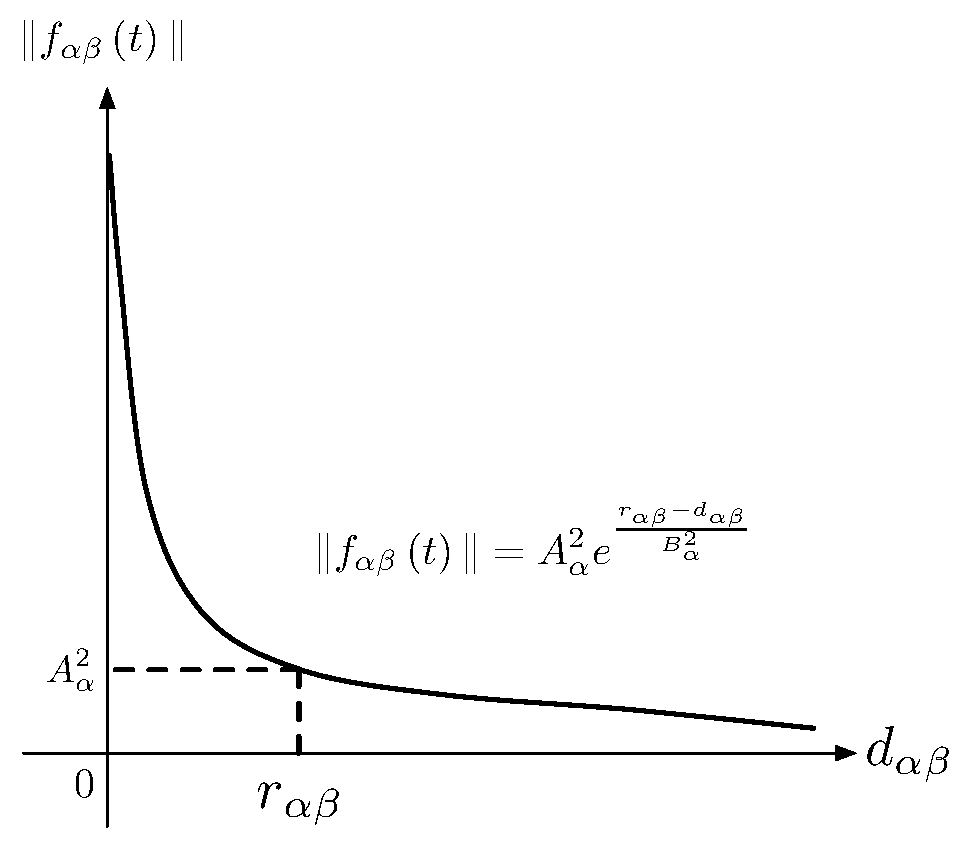
\includegraphics[scale=0.45]{Figures/physicalinteraction.pdf} 
\caption{The function about the interaction force $\vec{f_{\alpha\beta}}(t)$ and the distance between two agents
$d_{\alpha\beta}$ }\label{fig:physicalinteraction}
\end{figure}

There is one intersection of the graph and the axis $ \left( 0, A_{\alpha}^{2} exp\left( \frac{r_{\alpha\beta} }{B_{\alpha}^{2}}\right)  \right)  $. If put into the constants, we will be able to get a maximum value of $ f_{\alpha\beta}(t) $, since the distance between agents cannot be negative. Here we set $ A_{\alpha}^{2} = 3 m/s^{2} $, $ r_{\alpha\beta} = 0.6 m $, and $ B_{\alpha}^{2} = 0.2 m $, so $ f_{\alpha\beta}(t)^{max} \doteq 60 m/s^{2} $, which is about six times the gravitational acceleration and represents a rather large force between agents (as large as six person's weight). \\\\
However, we notice that the effective part of the force calculated above is only the horizontal 
component that enables the agent to move horizontally in the plane where we do the simulation, 
but the reality is that the agents sometimes are also able to move vertically, for example, 
by stepping upon other people when they cannot take the pushing force from the surrounding agents. 
When that happens, the horizontal component of the repulsive force becomes smaller even if 
$d_{\alpha\beta}$ is kept the same.	
Therefore, a qualitative modification of dependence between $ f_{\alpha\beta}(t) $ and $ d_{\alpha\beta} $ could be:
\begin{figure}[hb]   
\centering
    {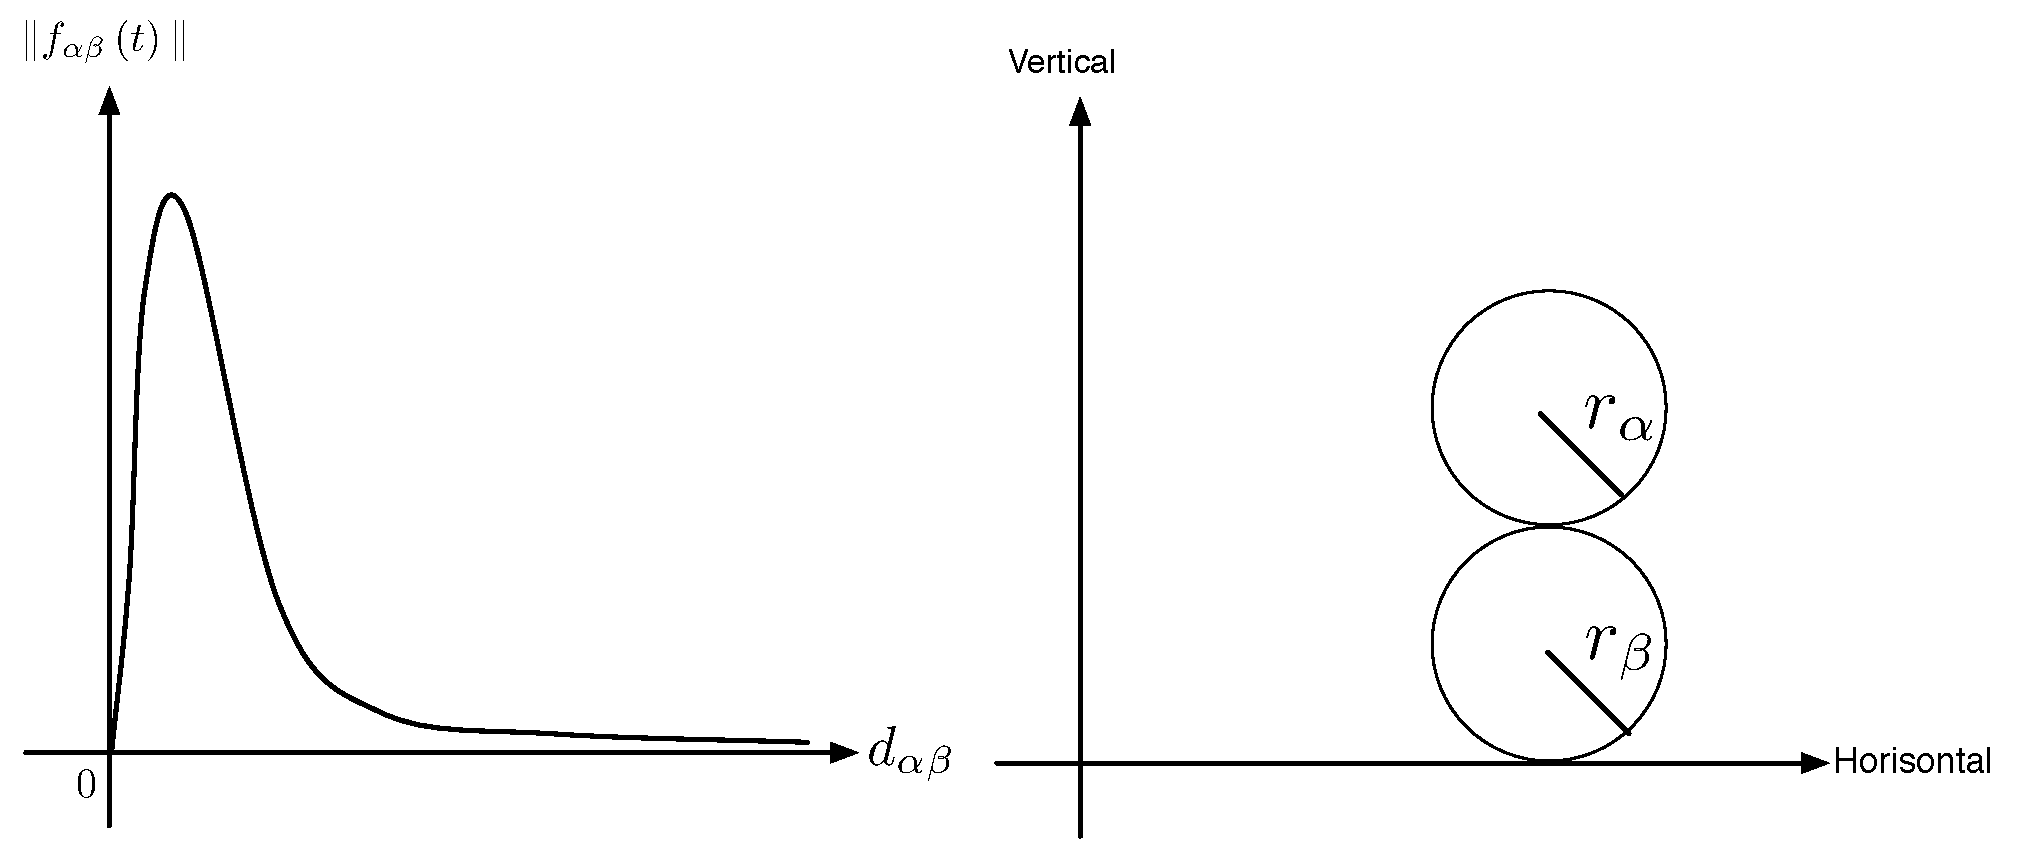
\includegraphics[scale=0.35]{Figures/ForceOverlapping.pdf}} 
    \caption{}
    \label{forceoverlapping}
\end{figure}
\\
\subsection{Use social force in further calculation}
use the value of forces to predict, as they are partly not real forces, the measurement does not reflect the reality in some range.
Pressure
